\section{Userspace variant based on NetfilterQueue}
\label{appfw:daf}

%%%%%%%%%%%%%%%%%%%%%%%%%%%%%%%%%%%%%%%%%%%%%%%%%%%%%%%%%%%%%%%%%%%%%%%%%%%%%%%%
\subsection{Problem statement}
\label{apffw:daf:intro}

In this first iteration of our distributed firewalling solution, we consider the
following research questions:

\textbf{RQ1: Reliable endpoint data source for NGFWs?} Micro-segmentation is a foundational component of zero-trust architectures. In contrast to traditional methods such as VLANs, micro-segmentation ensures network compartmentalization based on application layer visibility. However, most solutions today rely on the application classification features of NGFWs. We propose that one method of alleviating the over-reliance on TLS traffic decryption is by providing a pertinent, alternative data source that can uniquely identify endpoint applications and correctly associate this information with intercepted packets.

\textbf{RQ2: Compatibility with loosely defined networks?} In keeping with initiatives such as BeyondCorp, we take into account the fact that users could not only transition between internal networks, but also access resources from beyond the conventional network perimeter. As a result, we adopt a stateless Layer 3 traffic annotation mechanism and discuss possible improvements with regard to public network traversal.

\textbf{RQ3: Impact on network integrity and performance?} Ideally, a solution to the previous two questions would have minimal impact on both the network and individual hosts. Although certain concessions can ofttimes be made in favor of better security guarantees, we acknowledge the necessity for unobtrusive integration with pre-existing software stacks, as well as marginal downgrades in throughput. To this end, we aim to provide a prototype that is easily tunable to fit the unique requirements of each user.

In order to address these questions we propose \daf{}, a distributed application firewall \cite{ioannidis2000implementing} prototype capable of filtering traffic based on application identity. Its main characteristics are as follows:

\textbf{Originating process identification:} In contrast to existing solutions, we adopt a more discerning stance on how we distinguish applications from one another. We do not simply rely on the content extracted from processed packets to infer the identity of the originator. Instead, we determine all processes that had access to the socket that was used to emit a certain packet (a common occurrence in highly complex applications). Moreover, we are able to account for any object that was mapped in the virtual address space of said processes and use them as rule matching criteria. This approach is motivated by recent advances in attaining reproducible builds \cite{butler2023business} for both open and closed source software. One application of this feature is the ability to filter traffic that originated from processes that use a known vulnerable version of a certain library (e.g. \texttt{libssl} for traffic encryption). Alternatively, whitelists can be defined based on sets of binaries that comprise specific applications.

\textbf{Packet annotation:} In order to communicate that a packet had passed through \daf{} on the originating endpoint, we attach a Message Authentication Code (MAC). The MAC is embedded into the packet as an IP option, making our system connectionless. This allows the destination endpoint or any middleboxes that are aware of this annotation scheme to verify the authenticity of the received traffic. Alternatively, we attach an aggregate hash of all memory-mapped objects that comprised the originating process. This latter approach has a number of practical uses, e.g. allowing a system administrator to dictate the exact application and version one process is allowed to communicate with. Another function that could be served is that of a more general and reliable replacement of user-agent identification.

\textbf{Compatibility with container-based isolation:} Due to the widespread adoption of microservice architectures, we deemed it necessary to ensure that \daf{} could function across namespace boundaries. As a result, we demonstrate that our firewall can apply fine-grained filtration rules in Docker-based environments. This approach has the added benefit of isolating the firewall process from potentially malicious processes, to a certain degree.

We claim the following contributions:

\begin{itemize}
    \item The implementation of \daf{} \footnote{Code available at \url{https://github.com/RaduMantu/DAF}}, a network firewall capable of filtering and authenticating traffic based on the identity of the endpoint processes, regardless of namespace isolation.

    \item The integration of \daf{} with pre-existing firewalls (\texttt{iptables}) and Intrusion Prevention Systems (\texttt{snort3}), illustrating its potential for interoperability with existing traffic filtering technologies.

    \item An analysis of the inherent limitations of \texttt{NetfilterQueue} and the optimization techniques necessary for achieving satisfying throughputs for both consumer grade hardware as well as datacenter environments.
\end{itemize}

%%%%%%%%%%%%%%%%%%%%%%%%%%%%%%%%%%%%%%%%%%%%%%%%%%%%%%%%%%%%%%%%%%%%%%%%%%%%%%%%
\subsection{Architecture}
\label{apffw:daf:architecture}

In this section we describe the architecture of \daf{}. A high-level overview of our solution can be seen in Figure \ref{appfw:daf:fig:sys-architecture}. In order to operate our firewall, the first step would be for an administrator to create a whitelist of all the applications and their particular type of traffic that is allowed to be emitted. \daf{} allows the creation of classic firewall rules, such as permitting communication to/from specific IPs or ports, but extends this capability in one significant way: allowing applications to only accept traffic from other \textit{specific} applications. Moreover, \daf{} can prevent attacks such as DNS rebinding by limiting the pool of accessible networked resources on a per-application basis. Once started, \daf{} begins to collect system-level event data, create a local system-state model, and process packets on behalf of the built-in firewall.

\begin{figure}[h]
    \centering
    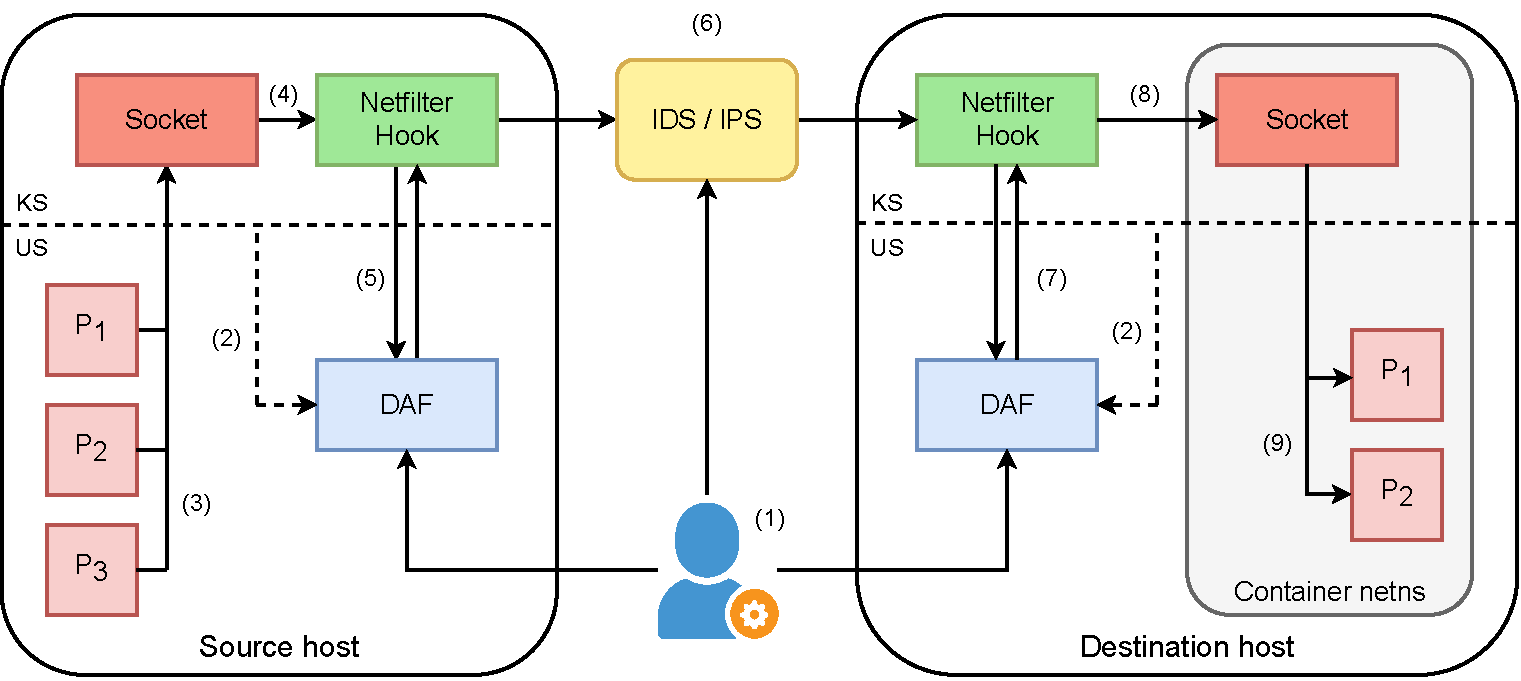
\includegraphics[width=\textwidth,keepaspectratio]{figures/daf-sys-architecture.pdf}
    \caption{Tagged packet data path. Both endpoints utilize \daf{}.}
    \label{appfw:daf:fig:sys-architecture}
\end{figure}

\subsubsection{Endpoint processes identification}
\label{appfw:daf:arch-endpoint}

In order to correlate a process with its specific network traffic, we have identified multiple possibilities:
\begin{itemize}
    \item When considering a threat model where the attacker has limited user-level privileges, \daf{} can be implemented as an extension to the current firewall mechanisms (e.g., \texttt{iptables}), with no intervention on the kernel. This is our main implementation detailed in this paper on Linux.
    \item If we assume an attacker with elevated privileges, \daf{} requires a kernel level implementation, similar with existing antivirus solutions. We have implemented this model on Windows as a proof of concept.
    \item Alternatively, if we regard the attacker as capable of gaining control of his immediate environment but unable to break container isolation, \daf{} can safely run in userspace, in a superior namespace.
    \item If we assume that the attacker has kernel-level privileges and there is no support for virtualization-based solutions, \daf{} can either be implemented on an external hardware token or in a Trusted OS. The former implies that network traffic can no longer be attributed to a certain process due to the lack to OS-level information, but can still be attributed to a certain host and prevent spoofing. Meanwhile, the latter would require hardware support for separating trusted and untrusted protection domains (e.g., ARM TrustZone). These use-cases are outside the scope of this paper.
\end{itemize}

%%%%%%%%%%%%%%%%%%%%%%%%%%%%%%%%%%%%%%%%%%%%%%%%%%%%%%%%%%%%%%%%%%%%%%%%%%%%%%%%
\subsection{Implementation}
\label{appfw:daf:implementation}

\subsubsection{Packet interception and modification}

There are multiple methods of intercepting, filtering and modifying network traffic. Our implementation is based on the \texttt{NetfilterQueue} extension to the \texttt{Xtables} system. \texttt{NetfilterQueue} takes advantage of the \texttt{nfnetlink\_queue} kernel subsystem to deviate packets that match \texttt{iptables} rules through a userspace process. This delegates the selection of built-in targets (i.e., ACCEPT, DROP, etc.) that are to be applied, to said process. Once the userspace process subscribes to a certain queue and starts receiving packets, these can be analyzed in full (starting with the Layer 3 header), further deferred for judgement to a different process and optionally, be arbitrarily modified before their eventual reintroduction in kernel space.

This approach permits us to implement \texttt{iptables} extensions without requiring the user to load any additional kernel modules. Considering that this system was initially introduced in August 2005 as part of Linux 2.6.14, it is safe to assume that most current-day distributions support this feature. Loading kernel modules on the other hand, while providing better performance due to the reduced number of context switches (exacerbated in \texttt{NetfilterQueue} by the lack of zero-copy), may be difficult to achieve on some virtual cloud environments due to the kernel being in lockdown. Our decision to extend \texttt{iptables} and not other firewall alternatives is motivated primarily by its prominence in the industry. For example, LinkedIn recently implemented a distributed firewall \cite{linkedin_dfw} that manages host-bound filtering rules based on \texttt{iptables} and its predecessor, \texttt{ipset}. Aside from the performance disadvantage, the main flaw that applies to \texttt{iptables} in general, and translates to our solution as well, is the possibility to bypass the Netfilter kernel hooks by using the \texttt{PF\_PACKET} low-level socket interface. However, this operation necessitates root privileges on the part of the attacker. Consequently, this particular scenario falls outside the purview of our threat model.


\subsubsection{Inferring process identity}

Correlating the information available in the headers of a packet with the process that emitted it is not a trivial task. The reason for this is the fact that identifying said process can only be done by instrumenting \texttt{sendmsg()} and other related system calls. By the time the payload effectively enters the network stack, the sought information would have already been lost. We ultimately decided that this option would necessit significant changes to the networking subsystem.

An alternative solution that we considered and ultimately decided to utilize involves correlating a selection of fields (e.g., source and destination IPs and ports) with the originating socket of the packet. We would subsequently use the inode of the socket to identify the processes that \textit{could} have sent the packet. Despite not being able to pinpoint the exact origin, this method gives a satisfactory approximation. All the information required for obtaining this mapping would normally be readily available to any \texttt{Xtables} rule match module that operates on the OUTPUT or POSTROUTING chains. However, it is not available on ingress. Since the destination socket is decided only after passing the PREROUTING and INPUT chain hooks and investigating the Layer 4 header, implementing this inference method as an \texttt{Xtables} extension would require a partial redesign of the Netfilter hook system.

We identified a different means to the same goal in the Netlink Socket Diagnostics subsystem. Originally designed as an alternative to \texttt{ioctl()} and an improvement over BSD routing sockets, Netlink sockets \cite{RFC3549} are used for Inter Process Communication (IPC) and facilitate interaction between userspace and certain kernel subsystems (e.g., sensor communication, packet routing/filtering rule manipulation, etc.) The Socket Diagnostics subsystem allows querying the kernel for specific socket-related information, including state and inode. This interface is preferred by tools such as \texttt{ss} over the older \texttt{procfs} alternative that \texttt{netstat} uses. Advantages include a binary communication channel (as opposed to the human-readable nature of \textit{/proc/net/*}), selective information retrieval and partial filtering based on characteristics such as local or remote IP addresses and ports.

Nonetheless, using the inode to identify the originating process of a packet raises a new challenge: socket file descriptors can easily be transferred between processes, and not only through inheritance on \texttt{fork()} or \texttt{clone()}. File descriptors can also be duplicated across processes using the ancillary \texttt{SCM\_RIGHTS} socket type. In early 2020, this procedure had been further simplified with the addition of a new system call capable of copying file descriptors from other processes, namely \texttt{pidfd\_getfd()}. Consequently, it would be ill-advised to regard only the original owner of the socket when deciding the identity of the sender. Instead, we must account for all open socket file descriptors, and their associated processes. Consequently, when evaluating an exclusionary match rule (i.e., DROP on object match), one process is sufficient to reach a verdict. Similarly, when we need to ensure that a certain version of a dependency is utilized, all potential originating processes must conform to the match criteria.

To this end, we trace a subset of system calls that are relevant for maintaining an accurate record of every socket that is accessible by one or more processes, as well as what those are. For example, \texttt{socket()} and \texttt{close()} may be relevant in following the activity of a single process. Meanwhile \texttt{fork()} or \texttt{clone()} compel us to copy the open file descriptors over to the child process in our model, by virtue of inheritance. This solution does not account for the system state prior to starting the firewall. As a result, we are prepared to perform a \texttt{procfs} walk and inspect the symbolic links in \texttt{/proc/<pid>/fd/} when the need arises (i.e., when a packet is matched to a socket of which we are unaware). Nonetheless, we do not expect this operation to be issued more than once. In order to perform this system call trace, we use two complementary mechanisms: eBPF tracepoints and the Netlink Process Event Connector subsystem. The former consists of analysis functions that are compiled to an eBPF target and uploaded into the kernel at runtime. If these programs pass the static validation stage, they are then attached to their respective tracepoints. Both the passed arguments and the return value are communicated to our firewall via a BPF ring buffer. Note that this mechanism is specific to \texttt{libbpf v1.0}, introduced with the \texttt{6.0} kernel release. This BPF ring buffer was first added in kernel version 5.8 and effectively supplanted the previous userspace communication medium (i.e.: the perf buffer) by reducing the number of senseless data copies and improving the event memory pool on SMP devices. We note that \texttt{libbpf v1.0} released on 22-Aug-2022, coinciding with the release of kernel version \texttt{6.0}. As a result of the deprecation of the pre-\texttt{v1.0} API, there is a possibility that \daf{} may not run correctly on older systems.

The latter tracing mechanism is yet another Netlink subsystem. The Process Event Connector is similar in function with eBPF probes, in that it reports system calls, including arguments, return values and the PID of the caller. We initially chose this tracing method due to encountering inconsistent behaviour in eBPF-based tracing of certain syscalls. The reason why we still use eBPF is that the Process Event Connector is only able to report on a very limited set of system calls, many falling outside its ambit. We note that one of the more significant drawbacks of the Process Event Connector is its lack of event filtering, meaning that extraneous events (e.g.: setting Effective User ID) can be discarded only after being received by the subscribed process.


\subsubsection{Filtering mechanism}

By using \texttt{NetfilterQueue}, the network traffic passes through two filtering stages (see Figure \ref{appfw:daf:fig:fw-architecture}). The first stage consists of the enforcement of the regular \texttt{iptables} rules. The second stage is entered only when one packet matches a rule with the \texttt{NFQUEUE} target. As a result of jumping to this target, the packet is passed to our userspace firewall instance for detailed analysis. The analysis is heavily reliant on the network socket utilization model that we continuously update. Specifically, the firewall needs to guarantee the availability of a list of processes that could have generated the packet (on egress) or are ready to receive the packet (on ingress). Similarly to \texttt{iptables}, \daf{} implements three chains: \texttt{INPUT}, \texttt{OUTPUT} and \texttt{FORWARD}. A \daf{} rule also consists of match criteria and a verdict. While the verdict can only be \texttt{ACCEPT} or \texttt{DROP}, the match criteria can be more complex, in comparison.

\begin{figure}[h]
    \centering
    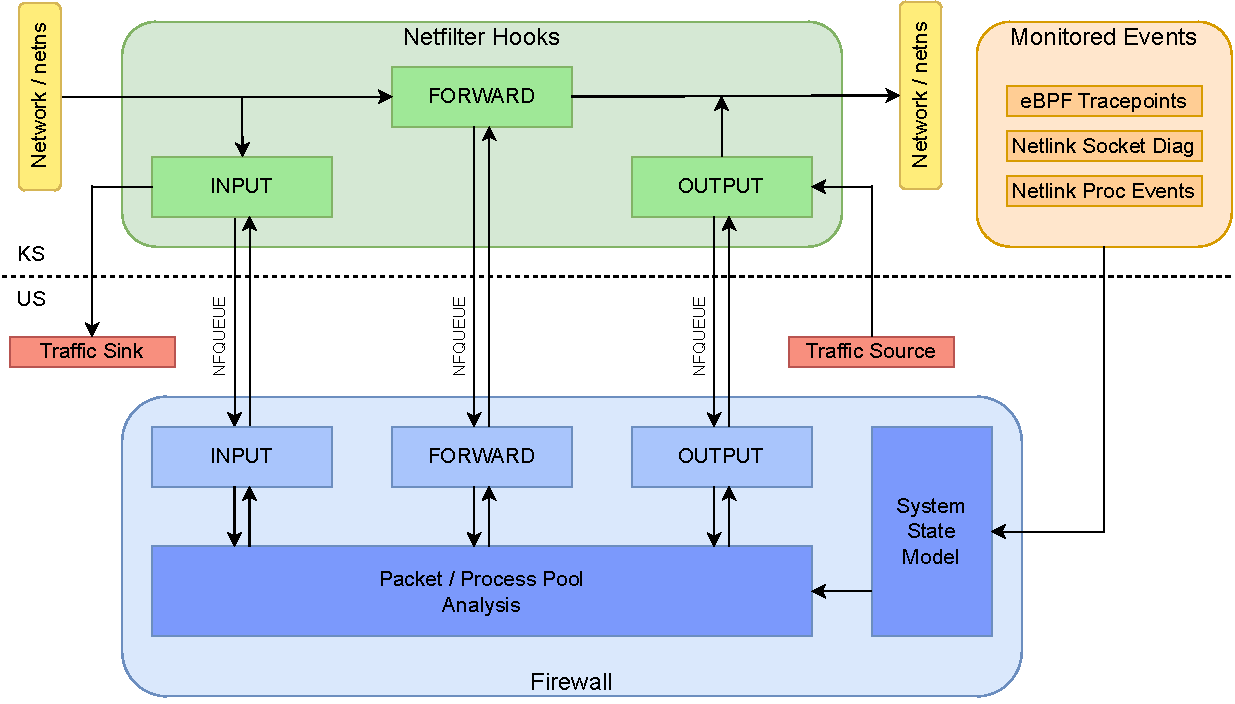
\includegraphics[width=\textwidth,keepaspectratio]{figures/daf-fw-architecture.pdf}
    \caption{Firewall architecture}
    \label{appfw:daf:fig:fw-architecture}
\end{figure}

The method we use the identity of a process to filter packets utilizes the objects mapped in its address space. The user can generate a rule requiring that a specific object (represented by its SHA256 digest) be either present or absent from all processes that are capable of generating or receiving the packets. Alternatively, the user can employ an aggregate hash of all file-backed objects with an executable section (sorted in alphabetical order on computation) to represent a specific version of a specific program, in a single rule. If the user wishes to issue a whitelist, then all processes must comply to this rule. Otherwise, if the user desires to enforce a blacklist, then a single process is sufficient to contravene the match criteria in order for the packet to be dropped.

The SHA256 digest itself is calculated based on the backing file of a memory mapped object, not on the in-process memory itself. The reason is twofold: monitoring memory access for every process without using static instrumentation is extremely costly, and excluding the writable sections to maintain the consistency of the digest gives leeway to an attacker. Although we assume that file permissions and ACLs are sufficient to protect the stored object files from tampering, one could extend \daf{} to monitor changes to hashed files via the inotify system.

Alongside the process identity matching mechanism, \daf{} also implements filtering based on IPs in CIDR notation, ports and Layer 4 protocol. These can all be configured by the \daf{} companion app, analogous to \texttt{iptables} itself. In addition to listing and managing rules, \daf{} is also capable of computing hashes and aggregate hashes for binaries and shared objects. This functionality was added to simplify the rule construction procedure.

\begin{lstlisting}[
    % style=bashstyle,
    caption={\daf{} rule configuration with companion app},
    label={appfw:daf:lst:rule}]
$ ctl-fw                                           \
    -A                  `# append rule           ` \
    -c OUTPUT           `# chain                 ` \
    -v DROP             `# verdict               ` \
    -d 192.168.100.0/24 `# destination IP        ` \
    -! --dport 80       `# (not) destination port` \
    -p tcp              `# L4 protocol           ` \
    -n /proc/$$/ns/net  `# network namespace     ` \
    --sng-hash $(sha256sum /usr/bin/curl           \
               | awk '{print $1}')
\end{lstlisting}

Listing \ref{appfw:daf:lst:rule} is an example of \daf{} rule that targets all local processes that run in the current network namespace and make use of the \texttt{curl} base binary. The rule prevents these processes from generating TCP traffic to ports other than 80 in a given subnet. For performing an exact match on \texttt{curl} in such way as to include its shared objects dependencies, the \texttt{-{}-agg-hash} flag can be used instead of \texttt{-{}-sng-hash}. Here, the companion app can be used to calculate the aggregate hash that should be passed as a parameter (see Listing \ref{appfw:daf:lst:hash}).

\begin{lstlisting}[
    % style=bashstyle,
    caption={Aggregate hash calculation},
    label={appfw:daf:lst:hash}]
$ ctl-fw $(ldd /usr/bin/curl \
         | awk '{print $3}'  \
         | xargs -L 1 echo -H)
/usr/lib/ld-linux-x86-64.so.2     -- 16d8048cc721c4...
/usr/lib/libbrotlicommon.so.1.1.0 -- c6bd47ce4931b2...
/usr/lib/libbrotlidec.so.1.1.0    -- 5989c61ae28cb2...
...
======================================================
AGGREGATE HASH                    -- e8f4f223875676...
\end{lstlisting}


\subsubsection{Support for Docker containers}

The isolation guarantees that a Docker container offers its user depends on a number of Linux primitives that can be employed individually to lesser effects, namely cgroups, namespaces and OverlayFS (supplanting \texttt{aufs}). When implementing container support in \daf{}, we tested our solution on a Dockerized proof of concept for CVE-2022-3602 (an \texttt{OpenSSL} buffer overflow that occurs during the X.509 certificate verification). We identified two distinct challenges:

\textbf{Resolving the absolute path of an object:} Because containerized processes utilize the mount namespace to an effect similar to that of \texttt{chroot}, the memory mapped objects present file paths that are relative to the mountpoint of the runtime OverlayFS layer. This mount is also called a \textit{merge directory} and offers access to the union of read-only \textit{lower} layers and the writable, instance-specific \textit{upper directory}. Assuming that \daf{} can access this mountpoint via its own filesystem (which is always the case if ran in the top-level namespace), resolving the absolute path becomes trivial. However, identifying the mountpoint can be achieved only by obtaining the mount options of the root filesystem that is used by the container. For OverlayFS, these options contain the paths to the lower, upper and merge directories and can be extracted from \texttt{/proc/<pid>/mountinfo}. Whenever we need to ascertain the identity of a process believed to have generated a matched packet, we first check whether it belongs to a different mount namespace. If so, we extract the path of the mountpoint (i.e., the \textit{merge directory}) and construct the absolute path of its objects.

\textbf{Contending with constrained socket diagnostics}: Although the Netlink Socket Diagnostics subsystem is the preferred method of identifying sockets based on Layer 3 and Layer 4 information, it has a severe limitation. The scope of any query is restricted to the network namespace that the calling thread is bound to. Because in this scenario the target process essentially belongs to another (virtual) subnetwork, the routing table must be consulted in order to first determine if the process in question even resides on the same system as the firewall and if so, what network namespace it is bound to. In this situation, we opted for a simpler solution: adding a required argument to each rule, explicitly stating the applicable network namespace. We deem this requirement to be reasonable, considering that this information should be readily accessible to a user with sufficient permissions and capabilities to configure \daf{}. Because the events that drive the continuous update of our system state model are not constricted by namespaces, once the socket inode is identified, the associated (real) PIDs can also be retrieved. This in turn provides the solution to the previous problem.

%%%%%%%%%%%%%%%%%%%%%%%%%%%%%%%%%%%%%%%%%%%%%%%%%%%%%%%%%%%%%%%%%%%%%%%%%%%%%%%%
\subsection{Evaluation}
\label{appfw:daf:evaluation}

\subsubsection{Experimental setup}

The experiments described in this section have been carried out on the following hardware:

\begin{itemize}
    \item \textbf{Intel NUC:} Intel Core i7-7567U CPU @3.50GHz, Intel I219-V 1-Gigabit Ethernet Controller, 8GB DDR4 memory @2400MT/s.
    \item \textbf{IBM System x3550 M4:} Intel Xeon E5-2650Lv2 CPU @1.70GHz, Intel 82599ES 10-Gigabit SFP+ Ethernet Controller, 32GB DDR3 memory @1600MT/s.
\end{itemize}

The reported throughput was derived from the \texttt{iperf3} output and was based on the application data transfer, excluding any headers. Both systems are running a minimal installation of Arch Linux with kernel version 6.7.0. We note that the \textit{rootfs} of the IBM server was network mounted. However, due to file buffering and file system syncs being transmitted on a different 1-Gigabit interface, this fact does not impact our experiments.

\subsubsection{Optimizations and trade-offs}
\label{appfw:daf:optimizations}

During the development of \daf{}, in an effort to achieve a satisfying performance, we were confronted with a number of potential trade-offs. Although some had the capacity to improve throughput by up to an order of magnitude, each would incur a reduction in our security guarantees. Consequently, we decided to implement these optimizations as either build-time or run-time user options. Following is a list of said optimizations, as well as their associated CLI invocation flag.

\begin{itemize}
    \item \textbf{Rescan prevention (R):} During the analysis of each packet, avoid scanning the virtual address space of each potential originator process, except during its initial identification. Subsequent queries will utilize the process state as it was ascertained during its first packet emission or reception. Dynamically loaded objects will not be accounted for.

    \item \textbf{Skip namespace switches (S):} Prevent switching network namespaces on consecutive rule evaluations that reference the same netns symlink. The symlink in question belonging to \textit{procfs} would not be an issue in and of itself. However, external references to said symlink are often used in order to prevent the kernel from deleting the namespace after all processes belonging to it have terminated. This principle can be found implemented in the \texttt{netns} subcommand of \texttt{iproute2}.

    \item \textbf{Disable cached object ordering (build-time; U):} In order to match packets using an aggregate hash that is representative for a certain program, the comprising objects must be arranged in a deterministic manner. To this end, we decided to sort them alphabetically based on their absolute paths. In our implementation, we cache the hashes of all objects belonging to a process as an unordered set, where operations have an average constant-time complexity. When retrieved by the Process Pool Analysis component, an ordered set (logarithmic complexity) is initialized from the contents of the unordered set, relying on its key comparison implementation to order the elements. During our experiments we discovered that we have initially underestimated the cost of this operation. As a result, we offer the choice of working directly with the unordered set in exchange for the ability to match whole programs, not just individual objects.

    \item \textbf{Batch verdict communication (b, B):} During our experiments we concluded that the packet data transfer between kernel space and user space is not a costly operation in and of itself. On the other hand, reporting the verdict for a given packet back to the \texttt{NetfilterQueue} module would block the process for what would at times amount to approx. 30\% of the total execution time. As a result, we decided to implement a verdict batching mechanism. Although capable of significantly improving the performance of \daf{}, we note that this optimization is not as straightforward to utilize as the previously described ones, its performance being contingent on the type of processed traffic. Thus, we define user-adjustable upper limits for both the number of batched packets, and the amount of time that the verdict of any packet is allowed to be delayed (see Subsection \ref{appfw:daf:queuq-verdict-batch-tuning}). Albeit difficult to suggest generic values that would guarantee an adequate performance increase regardless of the type of workload, we found it prudent to carry out forced verdict transmissions whenever a TCP SYN or TCP PSH is encountered. The reason behind the former is to avoid delaying the establishment of new TCP connections. As for the latter, postponing the transfer of what is expected to be a complete message to the endpoint process could provoke unwanted transmission delays at the application level.
\end{itemize}


\subsubsection{Netfilter Queue tuning}
\label{appfw:daf:queuq-verdict-batch-tuning}

When selecting the parameters for the \textbf{batched verdict communication optimization (b,B)}, we first determine the lower bounds for the maximum batch size and transmission timeout. Choosing the values for either of these parameters while falling short of this threshold can detract from the performance improvement of the optimization, to the point of completely negating it (e.g. size=1).

\begin{figure}[h]
    % Batch Size (b) impact on Throughput
    \begin{tikzpicture}
        % Throughput
        \begin{axis}[
            axis y line*      = left,
            width             = 0.9\textwidth,
            height            = 4.5cm,
            xmajorgrids       = true,
            ymin              = 4500,
            ymax              = 9500,
            xmin              = 1,
            xmax              = 50,
            xlabel            = {Batch size (b) [pkts]},
            ylabel            = {Throughput [Mbps]},
            % xticklabel style  = {rotate=45},
            xtick distance    = 5,
            ytick             = {5000, 7000, 9000},
            legend columns    = 3,
            legend entries    = {Min-Max throughput,
                                 Average throughput,
                                 Standard deviation},
            legend style      = {at={(-0.03,1.15)}, anchor=south west}
        ]
            % legend images (\addlegendentry fucks with fill plot)
            \addlegendimage{no marks, Green}
            \addlegendimage{no marks, RoyalBlue}
            \addlegendimage{no marks, Red}

            % Minimums and Maximums
            \addplot[name path=lower, color=Green, very thick]
                table[x=pkts, y=min, col sep=comma]
                {src/chapters/04-AppIdFirewall/data/batch-size.csv};
            \addplot[name path=upper, color=Green, very thick]
                table[x=pkts, y=max, col sep=comma]
                {src/chapters/04-AppIdFirewall/data/batch-size.csv};

            % Fill between Minimum and Maximum plots
            \addplot[pattern=north east lines,pattern color=Green] fill between[of=lower and upper];

            % Average
            \addplot[color=RoyalBlue, very thick]
                table[x=pkts, y=avg, col sep=comma]
                {src/chapters/04-AppIdFirewall/data/batch-size.csv};
        \end{axis}

        % Standard Deviation
        \begin{axis}[
            axis y line*      = right,
            x axis line style = {opacity=0},
            xmajorticks       = false,
            width             = 0.9\textwidth,
            height            = 4.5cm,
            xmin              = 1,
            xmax              = 50,
            % ymin              = 0.3,
            % ymax              = 2,
            ylabel            = {Std. Dev. [Mbps]},
        ]
            \addplot[color=Red, very thick]
                table[x=pkts, y=stdev, col sep=comma]
                {src/chapters/04-AppIdFirewall/data/batch-size.csv};
        \end{axis}
    \end{tikzpicture}

    % Batch Timeout (B) impact on Throughput
    \begin{tikzpicture}
        % Throughput
        \begin{axis}[
            axis y line*      = left,
            width             = 0.9\textwidth,
            height            = 4.5cm,
            xmajorgrids       = true,
            ymin              = 4500,
            ymax              = 9500,
            xmin              = 1,
            xmax              = 50,
            xlabel            = {Timeout (B) [$\mu{}s$]},
            ylabel            = {Throughput [Mbps]},
            % xticklabel style  = {rotate=45},
            xtick distance    = 5,
            ytick             = {5000, 7000, 9000},
        ]
            % Minimums and Maximums
            \addplot[name path=lower, color=Green, very thick]
                table[x=time, y=min, col sep=comma]
                {src/chapters/04-AppIdFirewall/data/batch-time.csv};
            \addplot[name path=upper, color=Green, very thick]
                table[x=time, y=max, col sep=comma]
                {src/chapters/04-AppIdFirewall/data/batch-time.csv};

            % Fill between Minimum and Maximum plots
            \addplot[pattern=north east lines,pattern color=Green] fill between[of=lower and upper];

            % Average
            \addplot[color=RoyalBlue, very thick]
                table[x=time, y=avg, col sep=comma]
                {src/chapters/04-AppIdFirewall/data/batch-time.csv};
        \end{axis}

        % Standard Deviation
        \begin{axis}[
            axis y line*      = right,
            x axis line style = {opacity=0},
            xmajorticks       = false,
            width             = 0.9\textwidth,
            height            = 4.5cm,
            xmin              = 1,
            xmax              = 50,
            % ymin              = 0.3,
            % ymax              = 2,
            ylabel            = {Std. Dev. [Mbps]},
        ]
            \addplot[color=Red, very thick]
                table[x=time, y=stdev, col sep=comma]
                {src/chapters/04-AppIdFirewall/data/batch-time.csv};
        \end{axis}
    \end{tikzpicture}

    \caption{Influence of verdict batch size \& timeout on throughput.}
    \label{appfw:daf:fig:batching}
\end{figure}


In order to empirically determine the aforementioned thresholds, we performed six rounds of experiments, varying the maximum batch size by 1 packet and the timeout by 1$\mu{}s$ in the 1-100 range (thus obtaining a dataset of 60,000 throughput values). Figure \ref{appfw:daf:fig:batching} illustrates the impact of each of the two tuning parameters via the average throughput on a 10Gbps link with constant MTU. In order to exemplify the effect of one tuning parameter independently from the other, the dimensions corresponding to the second parameter as well as the experiment round had to be collapsed. Consequently, each average throughput data point was calculated over a subset of 600 values representing the splice obtained from fixing the value on the abscissa.

For the minimum-maximum intervals we decided to fix both the experiment round and one of the tuning parameters, in order to then average the per-experiment minimums and maximums. The motive behind this was to de-emphasize outliers. To compensate for this and correctly represent the throughput variations, we included the standard deviation obtained from the same data slice that was used to calculate the average throughput. Here, we mention that the value range for both plots was truncated to 1-50 in order to better illustrate the impact of suboptimal parameter choices. The subsets used in the calculation of the average throughputs have not been proportionately truncated.

\begin{figure}[h]
    \begin{tikzpicture}
        \begin{axis}[
            width             = \textwidth,
            height            = 7cm,
            at                = {(0,0)},
            xmin              = 5500,
            xmax              = 9710,
            ymax              = 6300,
            xtick distance    = 1000,
            grid              = both,
            xlabel            = {MTU [bytes]},
            ylabel            = {Throughput [Mbps]},
            legend style      = {at={(0.04,0.80)}, anchor=west},
            legend cell align = left,
        ]
            \addplot[color=RoyalBlue, very thick]
                table[x=mtu, y=RUSuPb-doubling, col sep=comma]
                {src/chapters/04-AppIdFirewall/data/cocos-aliasing.csv};
            \addlegendentry{doubling}

            \addplot[color=LimeGreen, very thick]
                table[x=mtu, y=RUSuPb, col sep=comma]
                {src/chapters/04-AppIdFirewall/data/cocos-aliasing.csv};
            \addlegendentry{normal}
        \end{axis}
    \end{tikzpicture}

    \caption{Effect of introducing dynamic resizing of Netlink socket buffer.}
    \label{appfw:daf:fig:aliasing}
\end{figure}


One other value that we concluded needed to be fine tuned is the \textbf{Netlink socket receive buffer size}. While this socket is used for communication between userspace and the \texttt{Netfilter Queue} kernel driver, its receive buffer is also used to store packets that are pending a verdict, only to later be reintroduced in the network stack. In the eventuality that this buffer fills (a common occurrence when the userspace application is slow to reach a verdict) new packets are discarded and the following \texttt{read()} operation fails with the \texttt{ENOBUFS} error code, as an informative measure. Ignoring this problem can lead to aliasing issues that normally manifest as illustrated in Figure \ref{appfw:daf:fig:aliasing}. Insufficient TCP socket buffer sizes may also lead to similar performance downgrades. In response to these events, we assess the current Netlink socket buffer size and double it. This action is performed using the \texttt{SO\_RCVBUFFORCE} socket option as to override the system maximum socket size. We note that after doubling the buffer size from userspace, the kernel doubles it once more in order to allow for bookkeeping overhead.


\subsubsection{Performance analysis}

Our performance analysis of \daf{} is primarily based on \texttt{iperf3} throughput tests between a client running our firewall and a server on another identical host. The two hosts are directly linked, with no additional equipment serving as middleboxes. We note that the values we report represent the average throughput over 10s sessions, averaged once more over 10 and 5 rounds of experiments on the IBM server and NUC system respectively. On the 10-Gigabit servers, we decided to manually increase the default and maximum TCP socket buffer sizes, a common practice in such cases. Although in our final reports these are set to 32MB, we did not perceive any noticeable performance gain for values higher than 8MB. The NUC desktop computers utilize the default maximums of 4MB for the send buffer and 6MB for the receive buffer.

\begin{figure}[h]
    \centering

    \begin{tikzpicture}
        \begin{axis}[
            width             = \textwidth,
            height            = 6cm,
            at                = {(0,0)},
            xmin              = 600,
            xmax              = 9300,
            ymin              = 0,
            xtick distance    = 2000,
            grid              = both,
            xlabel            = {MTU [bytes]},
            ylabel            = {Throughput [Mbps]},
            legend style      = {at={(0.97,0.15)}, anchor=east},
            legend cell align = left,
        ]
            \addplot[color=RoyalBlue, very thick]
                table[x=mtu, y=sigRUS-usenix, col sep=comma]
                {src/chapters/05-SignatureFirewall/data/cocos-throughput.csv};
            \addlegendentry{RUS+sig (epoll)}

            \addplot[color=OliveGreen, very thick]
                table[x=mtu, y=sigRUS-esorics, col sep=comma]
                {src/chapters/05-SignatureFirewall/data/cocos-throughput.csv};
            \addlegendentry{RUS+sig (io\_uring)}
        \end{axis}
    \end{tikzpicture}

    \caption{\daf{} throughput on the IBM system with signature-based packet tagging.}
    \label{sign:linux:fig:cocos-throughput}
\end{figure}


Figure \ref{appfw:daf:fig:cocos-throughput} illustrates the performance gain of each optimization. Here, we note the exceedingly high variations. We attribute these to the use of the \texttt{io\_uring} interface for asynchronous I/O operations. In our implementation, we decided to launch a kernel thread on a different CPU core that continuously polls the system call submission queue in \daf{}. Prior to this revision, we employed an \texttt{epoll} hierarchization system to permit us the prioritization of certain events (e.g., system state model updates) over other. However, profiling sessions revealed that our firewall spent over 50\% of the time waiting for \texttt{epoll} events, limiting the average throughput with full optimizations to approx. 5.4Gbps. Our experimental results using this version can be found in Figure \ref{appfw:daf:fig:cocos-throughput-epoll}. In it there is an additional optimization, namely \textit{Uniform Prioritization (u)}. This optimization would circumvent the \texttt{epoll} hierarchy in order to give equal chances to both packets and system events to be processed, at the cost of potentially using an outdated system state when reaching a singular packet verdict. Once we transitioned to the \texttt{io\_uring} implementation, this optimization became redundant and was elliminated. As a reulst, bynot only offloading the majority of I/O operations (consisting mostly of packet reads from the netlink socket) to a secondary core but also drastically limiting the amount of context switches between protection domains, we have increased the average throughput to approx. 8.8Gbps. We believe that the gap between this and the baseline throughput can be bridged by extending \texttt{libnetfilter\_queue} to allow asynchronous batched verdict transmission.

\begin{figure}[h]
    \centering

    \begin{tikzpicture}
        \begin{axis}[
            width             = \textwidth,
            height            = 6cm,
            at                = {(0,0)},
            xmin              = 0,
            xmax              = 9710,
            ymin              = 0,
            ymax              = 6,
            xtick distance    = 1000,
            ytick distance    = 1,
            grid              = both,
            xlabel            = {MTU [bytes]},
            ylabel            = {Throughput [Gbps]},
            legend columns    = 7,
            legend style      = {at={(0.05,1.05)}, anchor=south west}
        ]
            \addplot[color=Goldenrod, very thick]
                table[x=mtu, y=baseline, col sep=comma]
                {src/chapters/04-AppIdFirewall/data/cocos-throughput.csv};
            \addlegendentry{baseline}

            \addplot[color=Rhodamine, very thick]
                table[x=mtu, y=vanilla, col sep=comma]
                {src/chapters/04-AppIdFirewall/data/cocos-throughput-epoll.csv};
            \addlegendentry{unopt}

            \addplot[color=Red, very thick]
                table[x=mtu, y=R, col sep=comma]
                {src/chapters/04-AppIdFirewall/data/cocos-throughput-epoll.csv};
            \addlegendentry{R}

            \addplot[color=Purple, very thick]
                table[x=mtu, y=RU, col sep=comma]
                {src/chapters/04-AppIdFirewall/data/cocos-throughput-epoll.csv};
            \addlegendentry{RU}

            \addplot[color=Green, very thick]
                table[x=mtu, y=RUS, col sep=comma]
                {src/chapters/04-AppIdFirewall/data/cocos-throughput-epoll.csv};
            \addlegendentry{RUS}

            \addplot[color=RoyalBlue, very thick]
                table[x=mtu, y=RUSu, col sep=comma]
                {src/chapters/04-AppIdFirewall/data/cocos-throughput-epoll.csv};
            \addlegendentry{RUSu}

            \addplot[color=Orange, very thick]
                table[x=mtu, y=RUSuPb, col sep=comma]
                {src/chapters/04-AppIdFirewall/data/cocos-throughput-epoll.csv};
            \addlegendentry{RUSuB}
        \end{axis}
    \end{tikzpicture}

    \caption{\daf{} throughput on IBM system (\texttt{epoll} version).}
    \label{appfw:daf:fig:cocos-throughput-epoll}
\end{figure}


In the same figure we also depict the throughput of \daf{} on the 10-Gigabit server while also calculating and attaching SHA256-HMACs of the Layer 4 payload as IP options. Notice how we forgo the use of verdict batching since it would not permit us to re-inject the modified packet into the kernel, strictly due to a \texttt{NetfilterQueue} API limitation. Once again, we believe that this limitation could be alleviated by adding a simultaneous packet override through an \texttt{iov} interface. However, this would also require changes not only to \texttt{libnetfilter\_queue} but also the \texttt{NetfilterQueue} driver, both of which we conside outside the scope of this paper. During this experiment we manually enforced a smaller Maximum Segment Size (MSS) for \texttt{iperf3} in order to ensure that the newly introduced 36-byte IP options section would not exceed the MTU at any given time. Note however, that \texttt{iperf3} clamps the MSS values within the 88-9216 range, thus leading to severe performance downgrades due to fragmentation. Under these conditions, we register a peak average throughput of approx. 835Mbps.

\begin{figure}[h]
    \centering

    \begin{tikzpicture}
        \begin{axis}[
            width             = \textwidth,
            height            = 7cm,
            at                = {(0,0)},
            xmin              = 600,
            xmax              = 2000,
            ymin              = 300,
            xtick distance    = 200,
            grid              = both,
            xlabel            = {MTU [bytes]},
            ylabel            = {Throughput [Mbps]},
            legend style      = {at={(0.97,0.15)}, anchor=east},
            legend cell align = left,
        ]
            \addplot[color=Goldenrod, very thick]
                table[x=mtu, y=baseline, col sep=comma]
                {src/chapters/05-SignatureFirewall/data/nuc-throughput.csv};
            \addlegendentry{baseline}

            \addplot[color=NavyBlue, very thick]
                table[x=mtu, y=RUSu-pktsig, col sep=comma]
                {src/chapters/05-SignatureFirewall/data/nuc-epoll-multiple.csv};
            \addlegendentry{RUS+sig (epoll)}

            \addplot[color=OliveGreen, very thick]
                table[x=mtu, y=sigRUS-esorics, col sep=comma]
                {src/chapters/05-SignatureFirewall/data/nuc-throughput.csv};
            \addlegendentry{RUS+sig (io\_uring)}
        \end{axis}
    \end{tikzpicture}

    \caption{\daf{} throughput on Intel NUC with signature-based packet tagging.}
    \label{sign:linux:fig:nuc-throughput-new}
\end{figure}


Observing the measurements on the Intel NUC mini-PC from Figure \ref{appfw:daf:fig:nuc-throughput}, we conclude that it is significantly easier to obtain near-linerate throughput both when annotating traffic and when only performing packet filtering. These results are in part due to the single CPU core speed, motivated by the fact that \daf{} is not multi-threaded. We note that the Intel driver for gigabit network adapters (i.e., \texttt{e1000e}) imposes a minimum MTU value of 604 bytes. Any attempt to set a lower value is met with a reset of the network interface, coupled with a silent override of the MTU, using this lower limit.

